\subsubsection{Normality}\label{subsubsec:hdassumptionsnormality}

For the residuals of the total number of collisions and the broadcast time the
normality is verified, as we can see from the QQ-plots: for these indexes we
always get \(R^2 > 0.93\).

The QQ-plot for the residuals of the percentage of covered users looks odd: this
is expected since the coverage can not go beyond \(100\%\) and the mean is
always near the maximum. Since we do not have studied the percentage of covered
users in \secref{subsec:hd2kr}, there is no need to verify the assumptions for
this index.

\figref{fig:hdmessagesqqplot} shows the QQ-plot for the residuals of the total
number of messages sent. We get \(R^2\!=\!0.8958\). This is caused by some
outliers on the left of the plot and the fact that the total number of messages
sent is superiorly limited by the total number of users in the network. Although
the normality is not perfect, it is still nearly normal.

\begin{figure}[htb]
	\centering
	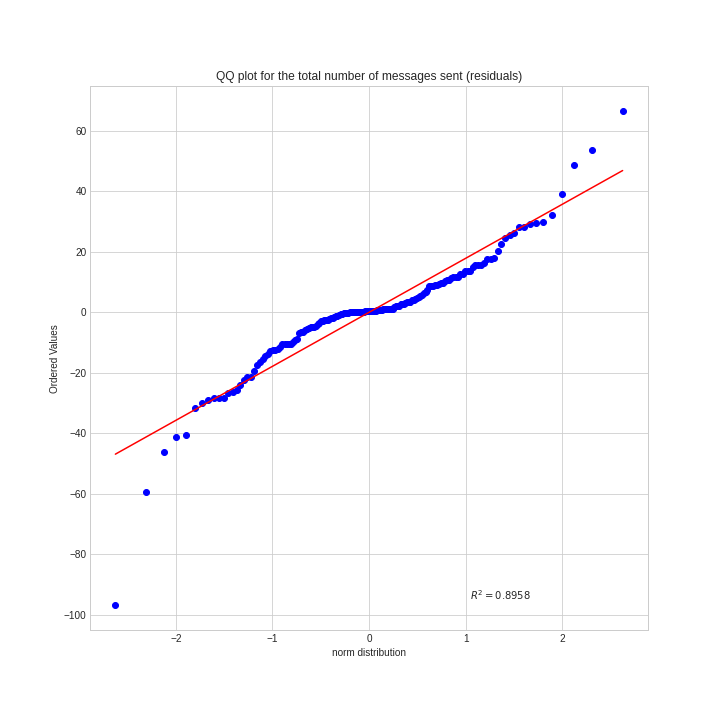
\includegraphics[width=0.77\textwidth]{img/hd/messages-qq}
	\caption{QQ-plot for the residuals of the total number of messages
	sent}\label{fig:hdmessagesqqplot}
\end{figure}
